\chapter{Optimalizace orientace faset}
	
\section{Postup optimalizace}
	Před tím, než přistoupíme k problému optimalizace, je třeba získat potřebná data. Důležité jsou informace o parametrech svazků, které lze rozdělit na \textit{simulované} a \textit{reálné}.

\subsection*{Simulované svazky}
\begin{enumerate}

\item 	Získáme potřebné parametry kamene, který zkoumáme. Zdrojem může být technický výkres, nebo předchozí měření.  

\item	Sestavíme model, který bude přibližně určovat tvar kamene. Tento model budeme považovat za \textit{referenční}.

\item	V programu LADOK simulujeme průlet svazku \textit{referenčním} modelem. Pro simulaci je důležité znát elektromagnetické vlastnosti laserového svazku a index lomu kamene. 

\item	Výsledkem simulace jsou parametry \textit{simulovaných} svazků.

\end{enumerate}

\subsection*{Reálné svazky}
Předpokladem pro získání parametrů \textit{reálných} svazků je sestavení a kalibrace měřicí soustavy podle \cite{Drapela}. % odkay na kapitolu
\begin{enumerate}

\item 	Opracovaný kámen umístíme do měřicí soustavy.

\item	Provedeme experiment průchodu svazku kamenem podobný situaci v simulačním programu LADOK. 

\item	Získáme obraz dopadu svazků na stínítko. 

\item	V obraze detekujeme světelné stopy (kapitola \ref{sec:detection}).  

\item	Z detekovaných stop vypočítáme parametry \textit{reálných} svazků (kapitola \ref{sec:beam parameters}).

\end{enumerate}

Přecházíme k situaci, kdy máme dostupné informace o \textit{simulovaných} i \textit{reálných} svazcích. Mezi těmito dvěma množinami je třeba nalézt korespondence. Korespondující svazky si odpovídají seznamem faset kamene, na které při své cestě dopadají.  

Pro korespondující páry určíme chybovou funkci a parametry budeme optimalizovat. Optimalizační algoritmus odhadne takové nastavení parametrů, aby bylo optimalizované kritérium co nejmenší. 

Optimalizované parametry použijeme k výpočtu \textit{optimalizovaného} modelu kamene. Orientace faset broušeného kamene odečteme z \textit{optimalizovaného} modelu.   

% diagram je vytvoren -> 500pm -> bitmap -> online to EPS -> latex to PDF -> load PDF
\begin{figure} [h!]
\centering
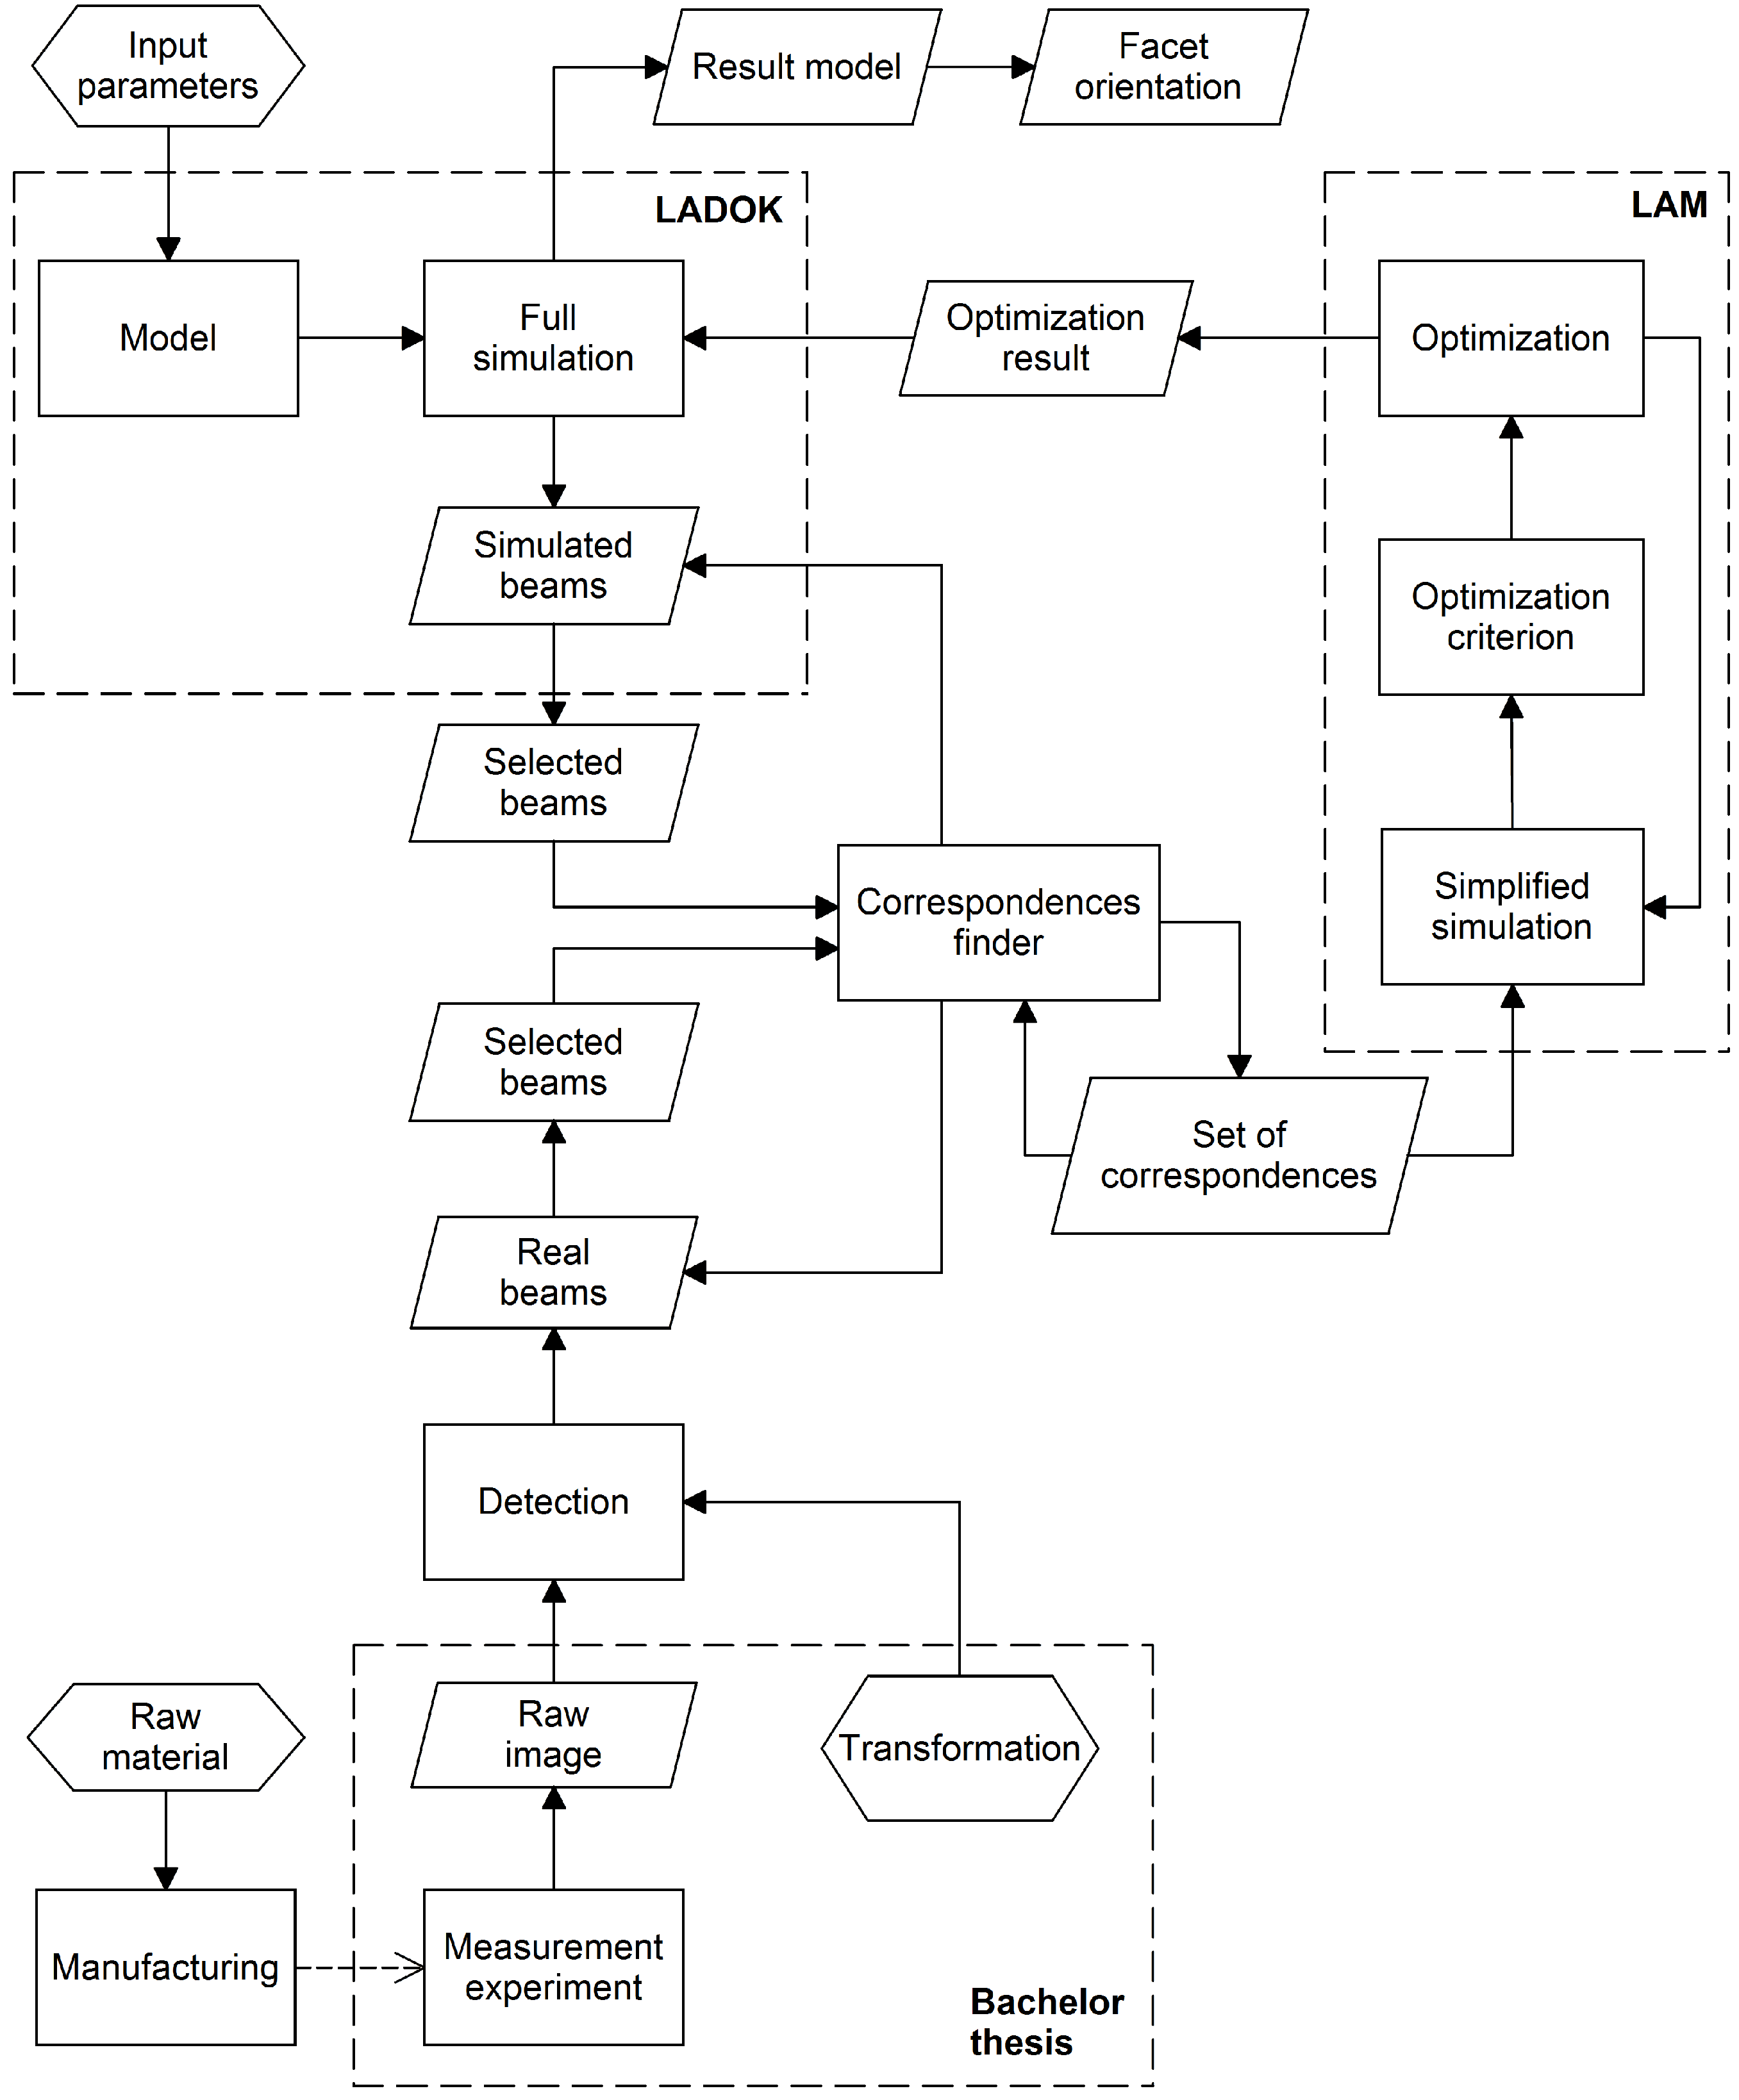
\includegraphics[width = \textwidth]{diagram.pdf}
\caption{Diagram with princip of cut stone facet orientation estimator.}
\label{fig:diagram}
\end{figure}

\clearpage

\section{Korespondence}

Zdrojový svazek odpadá na maximální možnou plochu kamene. Vlivem toho vystupuje z kamene velké množství svazků. Po dopadu svazků na stínítko je složité zpětně určit, které stopy náleží kterým svazkům.

\subsection{Podmíněnost}
Základní otázkou optimalizačního problému je, zda je systém dostatečně podmíněný. První podmínku, kterou musíme splnit je získat minimálně stejný počet nezávislých rovnic, jako je počet optimalizovaných parametrů. 

V optimalizačním kritériu máme celkem  $2\,r + q$ nezávislých rovnic. Základní podmínkou je, že počet korespondencí musí být minimálně $ s+q $.

To, jak dobře korespondující svazky podmiňují daný model do jisté míry závisí na počtu dopadových faset. Svazky s velkým počtem dopadových faset logicky 



Od tříd \textbf{1A} a \textbf{1B} lze obecně čekat velmi dobrou podmíněnost. Jednotlivý svazek z těchto tříd dopadne pouze na jednu fasetu a směr odraženého svazku jednoznačně určuje parametry fasety, od které se svazek odrazil. Pokud by máš matematický model přesně odpovídal reálnému experimentu, potom postačí nalézt korespondence třídy \textbf{1A} \textbf{1B}, abychom určili parametry všech faset kromě spodku. Tyto třídy nepodmiňují index lomu kamene, pokud bychom chtěli zjistit index
 
 
Teoreticky korespondencí svazků třídy \textbf{3A} (např. UF1-TOP-BOT) získáme 2 rovnice $\Delta e$ a $\Delta \alpha$, které jsou závislé na parametrech dopadových faset UF1, TOP a BOT. Problém spočívá v tom, že tato korespondence určuje pouze vzájemnou polohu dopadových faset a nelze u této třídy očekávat dobrou podmíněnost. 


\subsection{Výpočet odchylek parametrů}

1. možnost - kámen během optimalizace rotujeme. Výsledky rotace si zapamatujeme a odchylky faset budeme počítat vzhledem k parametrů faset rotovaného kamene. 

% je treba popsat, aby se tomu dalo rozumět
2.možnost - Kámen sice rotujeme a optimalizujeme, ale to nic nemění na tom, jak budeme počítat odchylky. Vezmeme si normály faset optimalizovaného a referenčního kamene. Nalezneme rotační matici mezi normálami spodku optimalizovaného a referenčního kamene. Rotační matici aplikujeme i na všechny ostatní fasety. Výsledkem bude to, že kamen srovnáme podle spodku. Chybové parametry pro spodek tak budou nulové.

Dále se postupuje tak, že se nalezne rotace mezi 

\subsection{Pozorování}

Simulujeme průlet světelného svazku optickým klínem (obr. \ref{fig:wedge}). Prostředí s indexy lomu $\eta_1$, $\eta_2$ a $\eta_3$ oddělují rozhraní $\rho_1$ a $\rho_2$. Tyto rozhraní mezi sebou svírají úhel $\alpha$.
\begin{figure}[h!]
\begin{center}
\scalebox{0.8}{ \input{xfig/mirror2.pstex_t}}
\end{center}
\caption{Lom a odraz paprsku v optickém klínu.}
\label{fig:wedge}
\end{figure}

\begin{equation}
\gamma = \arcsin{\left(\frac{\eta_1}{\eta_2}\sin{\beta}\right)}\,.
\end{equation}

\begin{equation}
\varepsilon_1 = \arcsin{\left(\frac{\eta_2}{\eta_1}\sin{\left(\gamma + 2\,\alpha\right)}\right)}\, 
\rightarrow \begin{cases}
\alpha > 0, & \varepsilon_3 > \varepsilon_2 > \varepsilon_1 > \beta\\
\alpha = 0, & \varepsilon_3 = \varepsilon_2 = \varepsilon_1 = \beta\\
\alpha > 0, & \varepsilon_3 < \varepsilon_2 < \varepsilon_1 < \beta
\end{cases}
\end{equation}


Svazek dopadá na rozhraní $\rho_1$ pod úhlem $\beta$. Na obrázku \ref{fig:wedge} je tento svazek reprezentován paprsek č.0. 

Svazek světla můžeme charakterizovat velikostí zářivého toku $\phi_e$. Z Fresnelových rovnic víme, že pokud na rozhraní $\rho_1$ nedochází k totálnímu odrazu, tak po dopadu svazku na rozhraní vznikne odražený a lomený svazek. Jaká bude velikost zářivého toku odraženého svazku $\phi_{e_{reflect}}$ závisí na polarizaci světla, dopadajícím úhlu a poměrem mezi indexy lomu prostředí, které odděluje rozhraní $\rho_1$.

\begin{equation}
\phi_e = \phi_{e_{reflect}} + \phi_{e_{refract}}\,.
\end{equation}

 Při dopadajícím úhlu $\beta = 0^\circ$ a indexech lomu $\eta_1 = 1$, $\eta_2 = 1.5$ se \SI{4}{\percent} dopadajícího zářivého toku odrazí. $\frac{\phi_{e_{reflect}}}{\phi_e} = 0.04$, $\frac{\phi_{e_{refract}}}{\phi_e} = 0.96$.

Z principu šíření světla optickým prostředím pozorujeme svazky 0 až 9, se specifickým směrem šíření. 

V šatonové růži nastává stejný optický jev mezi tabulkou (TOP) a spodkem (BOT), kde
\vspace{4mm}
\begin{tabular}{p{2cm} l}
$\eta_1$ & index lomu vzduchu,\\
$\eta_2$ & index lomu materiálu kamene,\\
$\eta_3$ & index lomu odrazivé vrstvy,\\
$\rho_1$ & tabulka\\
$\rho_2$ & spodek\\
\textbf{0} & zdrojový svazek,\\
\textbf{1} & svazek třídy \textbf{1B} - TOP,\\
\textbf{3} & svazek třídy \textbf{3B} - TOP-BOT-TOP,\\
\textbf{5} & svazek třídy \textbf{5E} - TOP-BOT-TOP-BOT-TOP,\\
\textbf{7} & svazek třídy \textbf{7H} - TOP-BOT-TOP-BOT-TOP-BOT-TOP,\\
\textbf{2,4,6,8} & tyto svazky nevznikají - na rozhraní $\rho_2$ dochází pouze k odrazu.\\
\end{tabular}
\vspace{4mm}

V reálné situaci nejsou fasety TOP a BOT rovnoběžné. Důsledkem toho svazky \textbf{1B}, \textbf{3B}, \textbf{5E} a \textbf{7H} svírají s normálou tabulky různý úhlem. Svazek třídy \textbf{3B} bude mít vždy největší zářivý tok. Zajímavé je, že tyto svazky leží ve stejné rovině. Tato rovina je určena vzájemnou orientací mezi normálou tabulky a normálou spodku.

Po dopadu svazků \textbf{1B}, \textbf{3B}, \textbf{5E} a \textbf{7H} na stínítko můžeme v obraze pozorovat stopy ležící na jedné přímce obr. \ref{fig:wedge_example_image}. 

\begin{figure} [h!]
\centering
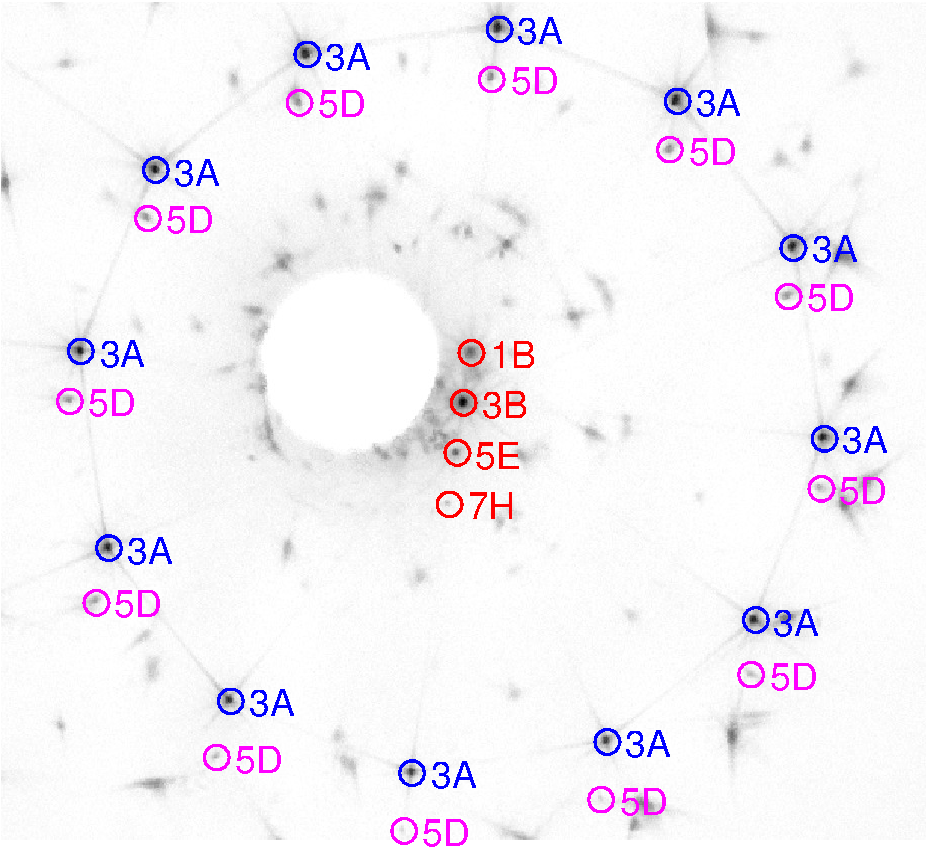
\includegraphics[width = 0.9\textwidth]{wedge_example.pdf}
\caption{Zvýraznění obrazů svazků ve snímku. Svazky třídy \textbf{1B}, \textbf{3B}, \textbf{5E} a \textbf{7H} dopadají pouze na fasetu TOP a BOT. Svazky třídy \textbf{3A} a \textbf{5D} dopadnou nejprve na boční fasetu a poté následuje jeden resp. dva dopady na dvojici faset BOT-TOP.}
\label{fig:wedge_example_image}
\end{figure}

 Pokud bychom byli schopni přiřadit alespoň 2 tyto stopy ke svazkům můžeme určit orientaci tabulky a spodku. Situaci ovšem komplikuje fakt, že ne vždy můžeme nalézt obrazy těchto stop, protože jsou zastíněny podstavcem, na který pokládáme kámen. 
 
 U svazků třídy \textbf{3A} a \textbf{5D} dochází k podobnému optickému jevu pouze s tím rozdílem, že svazek do kamene nevstupuje tabulkou, ale boční fasetou. Můžeme si všimnout stejné orientace obrazů dvojice svazků se stejnou vstupující fasetou. Tato dvojice také určuje vzájemnou orientací mezi normálou tabulky a normálou spodku. Pro jednoznačné této orientace je však nutné znát orientaci bočních faset.   

\section{Optimalizované kritérium}
\label{sec:Optimalizace_crit}
Optimalizační algoritmus je převzat z práce \cite{Bodlak2005}. Některé části byly pozměněny. Ukážeme si stručný přehled metody optimalizace a zvýrazníme provedené úpravy. Optimalizační algoritmus používáme nejen k odhadu parametrů faset kamene, ale také k odhadu indexu lomu kamene a jeho orientace kamene v měřené soustavě 

Definujeme kriteriální funkci, kterou budeme optimalizovat. Funkci lze popsat vztahem 

\begin{equation}
\vec{\varepsilon} = h\left(\vec{x},\vec{v},\vec{l},\vec{p} \right)\,,
\end{equation}

\begin{tabular}{l p{12cm}}
$\vec{p}$ & Obsahuje směrové vektory \textit{reálných} svazků. Směr popisujeme pomocí souřadnic azimutu a elevace. Pokud pro výpočet optimalizačního kritéria použijeme $s$ \textit{reálných} svazků, bude mít vektor $\vec{p}$ délku $2\,s$. \\ & \\

$\vec{l}$ & Obsahuje seznam dopadových faset svazku. Tento seznam je využit pro výpočet směru výstupního svazku. Délka seznamu se musí rovnat $s$. \\ & \\

$\vec{v}$ & Popisuje směr zdrojového svazku světla\\ & \\  

$\vec{x}$ & Vektor parametrů, které nastavuje optimalizační algoritmus.
\paragraph{Parametry faset, index lomu}

 Jedná se převážně o parametry $r$ uvolněných faset. Každou fasetu lze parametrizovat pomocí úhlové změny normálového vektoru $\vec{n}$ (2 parametry) a změny vzdálenosti $d$ fasety od souřadného systému (1 parametr).\\
& Optimalizační metoda nemá dostatečnou citlivost na změny vzdálenosti $d$ fasety \cite{Bodlak2005}. Tento parametr proto považujeme za konstantu.\\
& Nově lze mezi optimalizované parametry přidat index lomu kamene $n_i$. Celkově máme $2\,r + q$ parametrů, kde $q$ je 1 pokud je mezi $\vec{x}$ parametr $n_i$, jinak je $q$ rovno 0.

\paragraph{Orientace} Orientaci kamene popisujeme rotací kolem vertikální osy $R_z$ a dvou parametrů definujících náklon kamene $R_x$, $R_y$. 
 \\ & \\

$\vec{\varepsilon}$ & Představuje vektor odchylek v elevaci a azimutu \textit{simulovaných} a \textit{reálných} svazků.\\ 
& V práci \cite{Bodlak2005} byla tato odchylka měřena jako chyba v pozici dopadu laserového svazku na stínítku. Důvodem proč bylo využíváno toto kritérium byla citlivější odezva při změně vektoru svazku. Hlavním důvodem volby azimutu a elevace pro výpočet optimalizačního kritéria je vyšší rychlost. Odpadá totiž potřebný výpočet, který transformuje směrový vektor do souřadnic na stínítku.\\ & Vektor $\vec{\varepsilon}$ má $2\,s$ prvků.\\ & \\

\end{tabular}

\section{Plná vs. zjednodušená simulace}
V optimalizačním cyklu je použito dvou simulací, které simulují průlet světla broušeným kamenem

\subsection{Plná simulace}
Plnou simulací rozumíme klasický program LADOK, který modeluje odraz a lom svazků v konvexním tělese. Nevýhodou algoritmu je ale to, že simulace trvá příliš dlouho na to, aby mohla být úspěšně použita v optimalizačním procesu.

\subsection{Zjednodušená simulace}
Základní myšlenkou je, že se optimalizované parametry $\vec{x}$ příliš nemění. Za tohoto předpokladu si podstatná část svazků zachová posloupnost dopadových faset. Vynecháme proto kontrolu vzniku či zániku svazků. 

Zjednodušená simulace vyřadí z plné simulace zbytečné výpočty, které v procesu optimalizace nevyžíváme. 
Jediné, co potřebujeme znát je směr výstupních svazků. Pro výpočet směru nahradíme svazky nekonečně tenkými paprsky a můžeme s nimi pracovat jako s vektory. Fasety kamene reprezentujeme pomocí normálového vektoru. 

Zjednodušená simulace přistupuje k paprsku jednotlivě. Funkci pro výpočet vektoru výstupního paprsku $\vec{v_o}$ lze vyjádřit jako  

\begin{equation}
\vec{v_o}= g\left(\vec{v_i},\vec{N} \right)\,,
\end{equation}
kde $\vec{v_i}$ je vektor vstupního paprsku. Vektor $\vec{N}$ obsahuje normály $\vec{n_1},\dots,\vec{n_m}$ faset na které svazek dopadá. Normály jsou seřazené v pořadí odpovídající dopadovým fasetám při šíření paprsku od zdroje ke stínítku. 

Při výpočtu musíme vědět, která faseta svazek odráží a která lomí. Situace je jednoduchá. Pokud $m = 1$, potom muselo dojít k odrazu. Pokud  $m > 1$  odpovídají normály $\vec{n_1}$ a $\vec{n_m}$ fasetám, přes které se svazek lomí. Na ostatních fasetách se svazek odrazí. 







Zjednodušená simulace v LAMu pracuje s jinou funkcí. Základním rozdílem je to že navíc počítá polohu, kam paprsek na fasetu dopadl. Výpočet odrazu a jsou v LAMu pomalejší přibližně o \SI{15}{\percent}.

\section{Klasifikace příznaků}



\section{Implementace}
	Uvedeme algoritmy využité pro hledání korespondencí měřených a referenčních svazků a popíšeme jejich aplikaci pro automatické určení náklonu faset broušených kamenů. 
	Předtím, než se začneme zabývat navrženými přístupy, je třeba sjednotit značení jednotlivých parametrů svazků. 
	
	Referenční svazky dělíme do tří množin. 
	
	\begin{tabular}{l l}
	$\mathcal{R}_c$ & - uspořádaná $r_c$-tice svazků, pro které byl nalezen korespondující měřený svazek,\\
	$\mathcal{R}$   & - uspořádaná $r$-tice svazků, ke kterým můžeme přiřadit korespondující měřený savek, \\
	$\mathcal{R}_o$ & - uspořádaná $r_o$-tice svazků, které není možné přidat do množiny korespondencí $\mathcal{C}$.  \\
	\end{tabular}	

Pro tyto množiny platí $\mathcal{R}_c \cap \mathcal{R} = \emptyset$, $\mathcal{R} \cap \mathcal{R}_o = \emptyset$, $\mathcal{R}_c \cap \mathcal{R}_o = \emptyset$, kde $\mathcal{R} = \left(\mathrm{R}_1 ,\,\dots,\, \mathrm{R}_r\right)$. Dále definujeme uspořádanou $r^\prime$-tici $\mathcal{R}^\prime = \mathcal{R} \cup \mathcal{R}_o$. $r^\prime = r +r_o $.
	
	Podobně dělíme měřené svazky na $\mathcal{M}_c$, $\mathcal{M}$, $\mathcal{M}_o$ a $ \mathcal{M}^\prime$, kde $\mathcal{M} = \left(\mathrm{M}_1 ,\,\dots,\, \mathrm{M}_m\right)$.
	 
	 Algoritmy pracují s informacemi o směru, obrazu a zářivém toku $\phi_e$ svazků. Směr vyjadřujeme pomocí azimutu $\alpha$ a elevace $\varepsilon$. Polohu obrazu svazku určuje $x$-ová a $y$-ová souřadnice.
	
	 Parametry referenčních svazků označujeme $\vv{\alpha}_{r}$, $\vv{\varepsilon}_{r}$, $\vv{\phi}_{e_{r}}$, $\vv{x}_r$  a $\vv{y}_r$. Pro měřené svazky platí označení $\vv{\alpha}_{m}$, $\vv{\varepsilon}_{m}$, $\vv{\phi}_{e_{m}}$, $\vv{x}_m$  a $\vv{y}_m$. Platí, že $\vv{\alpha}_{r} = \alpha_{r}\left(\mathcal{R}\right)$, $\vv{\alpha}_{m} = \alpha_{m}\left(\mathcal{M}\right)$ apod. 

Množinu korespondujících svazků značíme $\mathcal{C}$. Jednotlivá korespondence $\mathrm{C}_i$ je uspořádaná dvojice $\left(\mathrm{R}_j,\,\mathrm{M}_k \right)$, $\mathrm{C}_i \subseteq \mathcal{C}$. $\alpha_{r}(\mathrm{C}_i)$ označuje azimut referenčního svazku $\mathrm{R}_j$, kde $\mathrm{R}_j \subset \mathrm{C}_i$ a $\alpha_{r}(\mathcal{C})$ vektor $\left(\alpha_{r}(\mathrm{C}_1),\,\dots,\,\alpha_{r}(\mathrm{C}_n)\right)$, kde $n$ je počet uspořádaných dvojic v množině $\mathcal{C}$.
	
	 

\subsection{Použité algoritmy}
	Korespondence hledáme buď pro specifickou třídu třídu svazků nebo pro svazky, které splní požadované parametry. 

\subsubsection{Korespondence svazků třídy \textbf{1A}}
\label{sec: 1A}

Víme, že svazky třídy \textbf{1A} se odráží od faset \textbf{UF1} - \textbf{UF2}. Úhlová odchylka normály referenční fasety skutečné normály se projeví dvojnásobnou úhlovou odchylkou referenčního svazku od měřeného. Očekáváme, že rozdíl mezi referenčními a reálnými parametry faset není příliš velký. Proto lze očekávat, že měřené svazky třídy \textbf{1A} budou mít velmi podobný směr jako referenční. Přibližně tedy známe směr těchto svazků.

V blízkém okolí stop třídy \textbf{1A} se mohou nacházet pouze stopy s řádově nižším zářivým tokem. Tato vlastnost je zajištěna geometrií kamene \textit{viva12} a provedením experimentu. Pokud známe zářivý tok stop, můžeme v obraze snadno nalézt svazek třídy \textbf{1A}. 

\paragraph{Parametry algoritmu}
\hspace{1mm}
	 
	 \begin{tabular}{l l}
	 $d_{max}$ & - kvadrát maximální vzdálenosti měřeného svazku od referenčního,\\
	 $n_{min}$ & - minimální počet měřených svazků, v blízkém okolí referenčního svazku, s nižším zářivým tokem než zářivý tok potenciálního korespondujícího měřeného svazku. \\
	 \end{tabular}
	
\paragraph{Popis algoritmu} 

\begin{enumerate}
\item Definujeme proměnné $\alpha_{c} = 0$, $\varepsilon_{c} = 0$, $\mathcal{C} = \emptyset$, $\mathcal{C}_{l} = \emptyset$.

\item $i = 0$.

\item Vypočítáme kritérium hodnotící vzdálenost mezi svazky 

$\vv{d} = (\alpha_{r}(\mathrm{R}_i)\cdot\vv{\mathbf{1}}-\vv{\alpha}_{m}-\alpha_{c}\cdot\vv{\mathbf{1}})^2 + (\varepsilon_{r}(\mathrm{R}_i)\cdot\vv{\mathbf{1}}-\vv{\varepsilon}_{m}-\varepsilon_{c}\cdot\vv{\mathbf{1}})^2 $.

\item Vybereme uspořádanou $k$-tici svazků $\mathcal{N}$ z $\mathcal{M}$, která odpovídá rostoucí posloupnosti $\vv{d}$ a omezení na $\vv{d} < d_{max}$. $\mathcal{N}_1 \sim \argmin(d)\,$ tak, že $\mathcal{N} = \left(\mathrm{M}_a ,\,\dots,\, \mathrm{M}_b \right)$, kde $a = \argmin(\vv{d})$ a $b = \argmin\left(\dfrac{1}{\vv{d}-d_{max}}\right)$. Dále bude platit, že  $\mathrm{N}_1 = \mathrm{M}_a$ a $\mathrm{N}_k = \mathrm{M}_b$ apod. 

\item Nalezneme uspořádanou $k$-tici $\mathcal{O}$ takovou, že $\mathcal{O} = \left(\mathrm{N}_1 ,\,\mathrm{N}_e,\,\mathrm{N}_f ,\,\dots,\, \mathrm{N}_g \right)$, kde\\$e = \argmin\left( \phi_{e_{m}}\left(\mathrm{N}_1 \right),\, \phi_{e_{m}}\left(\mathrm{N}_2 \right)  \right)$, $f = \argmin\left( \phi_{e_{m}}\left(\mathrm{N}_1 \right),\, \phi_{e_{m}}\left(\mathrm{N}_2 \right),\, \phi_{e_{m}}\left(\mathrm{N}_3 \right)   \right)$ a \\  $g = \argmin\left( \phi_{e_{m}}\left(\mathrm{N}_1 \right),\,\dots,\, \phi_{e_{m}}\left(\mathrm{N}_k \right)  \right)$.  

\item Určíme vektor $\vv{n_\mathcal{O}}$ o velikosti $k$ udávající četnost prvků z množiny $\mathcal{N}$ v množině $\mathrm{O}$. Pokud $\mathrm{O}_q = \mathcal{O}_s$, tak $n_{\mathcal{O}}(q) = n_{\mathrm{O}}(s)$, pro $q = \lbrace1,\,\dots,\,k \rbrace$ a podobně $s = \lbrace 1,\,\dots,\,k \rbrace$.

\item Určíme minimální $l$, které splňuje alespoň jednu z podmínek $n_{\mathcal{O}}(l) > n_{min}$  a $l = k$. Do množiny $\mathcal{C}$ přidáme korespondenci $\left(\mathrm{R}_i,\,\mathrm{N}_l \right)$.

\item Pokud $i \neq r$, tak $i = i+1$ a opakujeme body 3) až 7).

\item Pokud $\mathcal{C}_{l} \neq \mathcal{C}$, vypočítáme korekční parametry $\alpha_{c} = median(\alpha_{r}(\mathcal{C})-\alpha_{m}(\mathcal{C}))$, \\ $\varepsilon_{c} = median(\varepsilon_{r}(\mathcal{C})-\varepsilon_{m}(\mathcal{C}))$, položíme $\mathcal{C}_{l}$ rovno $\mathcal{C}$  a opakujeme body 2) až 8).

\item Z $\mathcal{C}$ odstraníme prvky, ve kterých se obraz referenčního svazku nachází mimo obraz stínítka.

\item Optimalizujeme náklon kamene (kapitola \ref{sec:Optimalizace_crit}).

\item Podle výsledku optimalizace upravíme model kamene a přepočítáme parametry referenčních svazků. Opakujeme bod 1) až 10). V příští iteraci tento bod vynecháme. 

\item Z $\mathcal{C}$ odstraníme prvky, ve kterých se obraz referenčního svazku nachází mimo obraz stínítka.

\end{enumerate}
\newpage
\subsubsection{Korespondence svazků třídy \textbf{3A}}	
\label{sec:3A}
	Po optimalizaci podle třídy \textbf{1A} máme dobře odhadnuté parametry faset \textbf{UF1} - \textbf{UF12}. Pomocí rotace a náklonu kamene odhadneme přibližně parametry faset \textbf{TOP} a \textbf{BOT}. Podstatné je, že svazek třídy \textbf{3A} dopadá na tabulku \textbf{TOP} pod výrazně menším úhlem, než je kritický úhel. To zajišťuje přijatelnou citlivost směru svazků na změnu parametrů dopadových faset. 
	
	Referenční svazky třídy \textbf{3A} mají po třídě \textbf{3B} druhý nejvyšší zářivý tok. Ostatní třídy se vyznačují řádově nižším zářivým tokem. Podle zářivého toku $\phi_{e_r}$  lze tedy snadno oddělit svazky se třemi dopadovými fasetami od ostatních svazků. Referenčních svazků třídy \textbf{3A} a \textbf{3B} je celkem 13. Často nastává situace, že svazek třídy \textbf{3B} nedetekujeme, protože je jeho obraz zakrytý podstavcem na kámen. 
	
	Separaci podle zářivého toku  však nelze s jistotou použít u měřených svazků. Pokud dojde k překrytí obrazu svazků jiných tříd, může být zářivý tok tohoto shluku větší. Spolehlivý způsob, jak oddělit měřené svazky třídy \textbf{3A} a \textbf{3B} od ostatních, je porovnat maximální úrovně jasu v obrazech svazků.  
	
	Další vlastnost, která dobře charakterizuje svazky třídy \textbf{3A} jsou dlouhé a intenzivní ocásky. Při hledání korespondencí můžeme využít párování svazků podle charakteru ocásků (kapitola \ref{sec: korespondence_ocasky}). Výhodou algoritmu je to, že dokážeme za vhodného nastavení nalézt korespondující svazky, a to i v případě vysokých směrových odchylek svazků. Nevýhodou je necitlivost na ostatní parametry svazků. 

\paragraph{Popis algoritmu} 

\begin{enumerate}
	\item Redukujeme počet měřených svazků a vytvoříme uspořádanou 13-tici $\mathcal{M}$ obsahující prvních 13 měřených svazků s nejvyšší hodnotou jasu v obraze. 

	\item Podle podobnosti ocásků nalezneme počáteční odhad množiny korespondencí $\mathcal{C}$ (kapitola \ref{sec: korespondence_ocasky})). Parametry algoritmu: $\sigma = 0.2$, $L_{min} = 2$, $\Delta\alpha_{max} = 35^\circ$, $\Delta\varepsilon_{max} = 15^\circ$.
	
	\item Uvolníme pouze parametry faset \textbf{TOP} a \textbf{BOT}. V tomto kroku prohlásíme parametry těchto dvou faset za totožné a optimalizujeme parametry uvolněných faset (kapitola \ref{sec:Optimalizace_crit}). Pokud neznáme dostatečně přesně index lomu kamene optimalizujeme také index lomu. 
	
	\item Podle výsledku optimalizace upravíme model kamene a přepočítáme parametry referenčních svazků. Pro finální odhad množiny korespondencí $\mathcal{C}$ použijeme algoritmus v kapitole \ref{sec: 1A} od bodu 1) do bodu 10). $\mathcal{R}$ bude uspořádaná 24-tice referenčních svazků třídy \textbf{1A} a \textbf{3A}. $\mathcal{M}$ bude obsahovat všechny měřené svazky.  
	
	\item K optimalizovaným parametrům přidáme parametry faset \textbf{UF1} až \textbf{UF12} a optimalizujeme. 
		
\end{enumerate}

\newpage
\subsubsection{Korespondence svazků třídy \textbf{5D}}
\label{sec:5D}
	Svazky třídy \textbf{5D} můžeme v obraze pozorovat, pokud existuje úhlová odchylka mezi fasetou \textbf{TOP} a \textbf{BOT}. Předpokládáme, že pokud nějaká odchylka vznikne, bude max. \SI{1}{\degree}. Také předkládáme, že normály faset \textbf{UF1} až \textbf{UF12} nejsou vůči pravidelnému tvaru \textit{vivy12} příliš vychýleny.
	
	Podstatné je, že známe polohu svazků třídy \textbf{3A}. Za výše uvedených okolností lze pozorovat vzor určující vzájemnou polohu dvojice svazků třídy \textbf{3A} a \textbf{5D}, které mají v seznamu stejné dopadové fasety např. dvojice (UF1-TOP-BOT, UF1-TOP-BOT-TOP-BOT). Vzájemnou polohu mezi všemi těmito páry lze popsat pomocí polárních souřadnic vzdáleností $\rho$ a úhlem $\varphi$. 
	
	Polohu j-tého měřeného svazku popisujeme souřadnicemi $x_m(\mathrm{M}_j)$ a $y_m(\mathrm{M}_j)$. Měřené svazky rozdělíme na uspořádanou $n$-tici $\mathcal{N}$ obsahující 12 svazků třídy 3A a uspořádanou $o$-tici $\mathcal{O}$ obsahující zbylé svazky. 

\paragraph{Parametry algoritmu}
\hspace{1mm}

	 \begin{tabular}{l l}
	 $\rho_{max}$ & - maximální vzdálenost obrazu svazků třídy \textbf{3A} a \textbf{5D} v pixelech,\\
	 $\Delta\rho$ & - maximální absolutní odchylka úhlu v obraze mezi párem svazků třídy \textbf{3A} a \textbf{5D},\\
	 $\Delta\varphi$ & - maximální absolutní odchylka vzdálenosti v obraze mezi párem svazků třídy \textbf{3A} a \textbf{5D},\\
	 $p_{min}$ & - minimální počet nalezených dvojic.\\
	 \end{tabular}

\paragraph{Algoritmus}

\begin{enumerate}
\item Vypočítáme Euklidovu vzdálenost obrazů jednotlivých svazků

$\rho_{j,k} = \sqrt{\left( x_m(\mathrm{N}_j) - x_m(\mathrm{O}_k) \right)^2 + \left( y_m(\mathrm{N}_j) - y_m(\mathrm{O}_k) \right)^2}$ 

pro $j = \lbrace 1,\,\dots,\,n \rbrace$ a $k = \lbrace 1,\,\dots,\,o \rbrace$. 

Směrový úhel určíme podle vztahu $\varphi_{j,k} = \arctan\dfrac{y_m(\mathrm{N}_j) - y_m(\mathrm{O}_k)}{x_m(\mathrm{N}_j) - x_m(\mathrm{O}_k)}$.

\item Vybereme svazky vzdálené méně než $\rho_{max}$ a dostaneme vektor vzdáleností $\vv{\rho}$ a směrových úhlu $\vv{\varphi}$.

$\lbrace \varphi_{j,k} \subseteq \vv{\varphi},\,\rho_{j,k} \subseteq \vv{\rho}\,|\,\, \rho_{j,k} < \rho_{max} \rbrace$ pro $j = \lbrace 1,\,\dots,\,n \rbrace$ a $k = \lbrace 1,\,\dots,\,o \rbrace$,
 
 kde  $\vv{\varphi} = (\varphi_{{j_1},{k_1}},\,\dots,\,\varphi_{{j_s},{k_s}}) = (\varphi_{1},\,\dots,\,\varphi_{s})$ a $\vv{\rho} = (\rho_{{j_1},{k_1}},\,\dots,\,\rho_{{j_s},{k_s}}) = (\rho_{1},\,\dots,\,\rho_{s})$. 

\item Definujeme funkce $g(x)\rightarrow \begin{cases}
1, & |x| < \Delta\rho\\
0, & jinak
\end{cases}\,, \hspace{4mm}h(x) \rightarrow \begin{cases}
1, & |x| < \Delta\varphi\\
0, & jinak
\end{cases}$. 

Pro vektor $\vv{x}$ délky $n$ platí $g(\vv{x}) = \left(g(x_1),\,\dots,\,g(x_n)\right)$ a $h(\vv{x}) = \left(h(x_1),\,\dots,\,h(x_n)\right)$.

 Nechť $a = \underset{{q = \lbrace1,\,\dots,\,s\rbrace}}{\argmax}\,\, \overset{s}{\underset{{i = 1}}{\sum}} g\left(\varphi_i-\varphi_q\right)$, \hspace{4mm} $b = \underset{{q = \lbrace1,\,\dots,\,s\rbrace}}{\argmax}\,\, \overset{s}{\underset{{i = 1}}{\sum}} h\left(\rho_i-\rho_q\right)$, potom 

$\vv{\upsilon} = g\left(\vv{\varphi} - \varphi_a\cdot\vv{\mathbf{1}} \right) + h\left(\vv{\rho} - \rho_b\cdot\vv{\mathbf{1}} \right)$.


\item Nalezeme množinu potenciálních korespondencí $\mathcal{C^\prime}$. $\lbrace \left(\mathrm{R}_t,\mathrm{O}_{k_q}\right) \subseteq \mathcal{C^\prime} \,|\,\, \upsilon_q > 1 \rbrace$, pro $q = \lbrace1,\,\dots,\,s\rbrace$, kde $R_t$ je referenční svazek třídy \textbf{5D} se stejným seznamem dopadajících faset jako měřený svazek $\mathrm{N}_{j_q}$.

\item Pokud $\mathcal{C^\prime}$ obsahuje alespoň $p_{min}$ prvků, přidáme $\mathcal{C^\prime}$ do množiny korespondencí $\mathcal{C}$.

 
\end{enumerate}

\newpage
\subsubsection{Korespondence svazků podle polohy v obraze a zářivého toku}
	Tento algoritmus se snaží o to nalézt dvojici svazků, které se promítnou na podobnou pozici v obraze a mají vysoký zářivý tok. Snažili jsme se nalézt funkci, která by charakterizovala závislost mezi zářivým tokem $\phi_{e_{r}}$ referenčních stop a zářivým tokem $\phi_{e_{m}}$ měřených stop. Jednoduchou funkci jsme však nenašli. Ke korespondenci svazků budeme místo absolutního zářivého toku využívat jeho relativní velikosti vzhledem k ostatním svazkům v blízkém okolí. 

\paragraph{Parametry algoritmu}
\hspace{1mm}

	 \begin{tabular}{l l}
	 $\rho_{max}$ & - maximální vzdálenost obrazu svazků třídy \textbf{3A} a \textbf{5D} v pixelech,\\
	 $\Delta\rho$ & - maximální absolutní odchylka úhlu v obraze mezi párem svazků třídy \textbf{3A} a \textbf{5D},\\
	 $\Delta\varphi$ & - maximální absolutní odchylka vzdálenosti v obraze mezi párem svazků třídy \textbf{3A} a \textbf{5D},\\
	 $p_{min}$ & - minimální počet nalezených dvojic.\\
	 \end{tabular}

\paragraph{Algoritmus}

\begin{enumerate}
\item $j = 1$, $\vv{w}_{m^\prime} = \vv{\mathbf{1}}$, $\vv{w}_{r^\prime} = \vv{\mathbf{1}}$. 

\item Nalezneme 3 svazky $\left(\mathrm{M}^\prime_a,\,\mathrm{M}^\prime_b,\,\mathrm{M}^\prime_c \right) \subset \lbrace \mathcal{M}^\prime\setminus \mathrm{M}^\prime_j\rbrace$ s nejmenší Euklidovou vzdáleností obrazu $\left(d_a,\,d_b,\,d_c\right)$ od svazku $\mathrm{M}^\prime_j$.

$d_a = \sqrt{\left( x_{m}(\mathrm{M}_j^\prime) -  x_{m}(\mathrm{M}_a^\prime) \right)^2 + \left( y_{m}(\mathrm{M}_j^\prime) -  y_{m}(\mathrm{M}_a^\prime) \right)^2}$.

\item Nechť $f(\mathrm{M}^\prime_x)\rightarrow \begin{cases}
\phi_{e_{m}}\left(\mathrm{M}^\prime_x \right), & d_x < d_{m_{max}}\\
1, & jinak
\end{cases}$, $\phi_{e_{m}}(\mathrm{M}^\prime_j) > 1 $ potom 

$\phi_{m^\prime_{max}} = \max\left(\phi_{e_{m}}(\mathrm{M}^\prime_j),\,f(\mathrm{M}^\prime_a),\,f(\mathrm{M}^\prime_b),\,f(\mathrm{M}^\prime_c)  \right)$. 

\item Nastavíme váhy měřených svazků.

 $w_{m^\prime_{q}} = \dfrac{\phi_{max}}{f(\mathrm{M}^\prime_q)}$ pro $q = \lbrace j,\,a,\,b,\,c \rbrace$.
 
\item Nalezneme uspořádanou $s$-tici $\mathcal{S} = (\mathrm{S}_1,\,\dots,\,\mathrm{S}_s)$ referenčních svazků z $\mathcal{R}^\prime$. 

$\lbrace \mathrm{R}^\prime_i \subseteq \mathcal{S}\,|\,\, d_{i,j} < d_{r_{max}}  \rbrace$ pro $i = \lbrace 1,\,\dots,\, r^\prime \rbrace$, kde 

$d_{i,j} = \sqrt{\left( x_{m}(\mathrm{M}_j^\prime) -  x_{r}(\mathrm{R}_i^\prime) \right)^2 + \left( y_{m}(\mathrm{M}_j^\prime) -  y_{r}(\mathrm{R}_i^\prime) \right)^2}$.

\item $w_{r^\prime_j} = max\left( \phi_{e_r}(\mathcal{S}) \right)$.

\item Dokud $j \neq n^\prime$, $j = j+1$ a opakujme body 2) až 6). 

\item Nechť  $g(x)\rightarrow \begin{cases}
x, & x > 1\\
1, & jinak
\end{cases}$, potom můžeme určit kriteriální funkci 

$\mathbf{L}(i,j) = d_{i,j}\cdot w_{m^\prime_{j}} \cdot g \left(\dfrac{\phi_{r_i}(\mathcal{R}^\prime_i)}{w_{r^\prime_{j}}} \right)$. 


\item Potenciální korespondence $\mathcal{C}^\prime$ nalezneme podle vzájemně nejnižší velikosti  kritéria v $\mathbf{L}$, které nepřekročí hodnotu $L_{max}$. Korespondující dvojice $\left(\mathrm{R}^\prime_i,\,\mathrm{M}^\prime_j \right) \subseteq \mathcal{C}^\prime$, pokud\\ $i = \underset{{q = \lbrace1,\,\dots,\,r^\prime\rbrace}}{\argmin}\mathbf{L}(q,j)$, $j = \underset{{q = \lbrace1,\,\dots,\,m^\prime\rbrace}}{\argmin}\mathbf{L}(i,g)$ a  $\mathbf{L}(i,j) < L_{max}$. 

\item Vybereme korespondence z $\mathcal{C}^\prime$, které můžeme přidat do množiny korespondencí $\mathcal{C}$. 

 $\lbrace \mathrm{C}^\prime_l \in \mathcal{C}\,|\,\, \mathrm{C}^\prime_l \subseteq \lbrace\mathcal{R}_f \cup \mathcal{M}_f\rbrace \rbrace$.

 
\end{enumerate}

\newpage
\subsubsection{Korespondence svazků podle ocásků}
\label{sec: korespondence_ocasky}
		
	Ocásky svazků definujeme pomocí velikosti a směrového úhlu.
	
	Počet ocásků referenčního svazku závisí na počtu stran polygonu, kterým popisujeme tvar svazku. Intenzitu ocásku v simulaci určuje zářivý tok svazku a na velikost hrany, na které ocásek vzniká. 
	
	Velikost $\vv{\xi}_{r}\left(\mathrm{R_i}\right)$ a směrový úhel $\vv{\psi}_{r}\left(\mathrm{R_i}\right)$ ocásků  $i$-tého referenčního svazku $\mathrm{R_i}$ určuje vektor o délce $n_i$.\\
	 $\vv{\xi}_{r}\left(\mathrm{R_i}\right) = \left(\xi_{r_1}\left(\mathrm{R_i}\right),\,\dots,\,\xi_{r_{n_i}}\left(\mathrm{R_i}\right)\right)$, $\vv{\psi}_{r}\left(\mathrm{R_i}\right) = \left(\psi_{r_1}\left(\mathrm{R_i}\right),\,\dots,\,\psi_{r_{n_i}}\left(\mathrm{R_i}\right)\right)$, kde $n_i$ je počet ocásků $\mathrm{R_i}$. 
	
	Detekce ocásků měřeného svazku je popsána v kapitole \ref{sec:tails}. Obecně platí, že v obraze jsou detekovatelné ocásky, pro které byla v odpovídající simulaci vypočítána vysoká intenzita. 
	
	Velikost ocásků $j$-té měřené stopy značíme $\vv{\rho}_{m}\left(\mathrm{M_j}\right)$, směrový úhel $\vv{\varphi}_{m}\left(\mathrm{M_j}\right)$. 
	 
	 Podobnost ocásků hodnotíme podle kritéria, a to především na základě podobnosti směru ocásků. Velikost ocásků určuje váhu jednotlivých příspěvků.
	 
\paragraph{Parametry algoritmu}
\hspace{1mm}
	 
	 \begin{tabular}{l l}
	 $\Delta\alpha_{max}$ & - maximální absolutní odchylka azimutu měřeného svazku od referenčního,\\
	 $\Delta\varepsilon_{max}$ & - maximální absolutní odchylka elevace měřeného svazku od referenčního,\\
	 $\sigma$ & - citlivost kriteriální funkce na úhlovou odchylku ocásků,\\
	 $L_{min}$ &  - minimální velikost kritéria  $\mathbf{L} \in \mathbb{R}^{r\times m}$ pro přidání dvojice svazků do množiny korespondencí $\mathcal{C}$. \\
	 \end{tabular}
	
\paragraph{Algoritmus}

\begin{enumerate}
\item $i = 1$

\item Normujeme velikost referenčních ocásků $\vv{\xi}_r\left( \mathrm{R_i} \right) = \dfrac{\vv{\xi}_r\left( \mathrm{R_i} \right)}{\max \left( \vv{\xi}_r\left( \mathrm{R_i} \right) \right)}\,.$

\item Z referenčních ocásků vybereme pouze ty s dominantní intenzitou a získáme vektor velikost $\vv{\rho}_{r}\left(\mathrm{R_i}\right)$ a směr $\vv{\varphi}_{r}\left(\mathrm{R_i}\right)$ o délce $n_k$.\\ $\lbrace \psi_{r_k}\left(\mathrm{R_i}\right) \subseteq \vv{\varphi}_{r}\left(\mathrm{R_i}\right),\, \xi_{r_k}\left(\mathrm{R_i}\right) \subseteq \vv{\rho}_{r}\left(\mathrm{R_i}\right)\,|\,\, \xi_{r_k}\left(\mathrm{R_i}\right) > \xi_{min} \rbrace$, kde $k =\lbrace 1,\,\dots,\,n_i\rbrace $.

\item Nalezneme uspořádanou $n$-tici $\mathcal{N}$ z měřených svazků $\mathcal{M}$. \\$\lbrace \mathrm{M}_j \subseteq \mathcal{N} \,\,|\,\,|\alpha_r(\mathrm{R}_i) - \alpha_m(\mathrm{M}_j) | < \Delta\alpha_{max},\, |\varepsilon_r(\mathrm{R}_i) - \varepsilon_m(\mathrm{M}_j) | < \Delta\varepsilon_{max} \rbrace$, kde $j =\lbrace 1,\,\dots,\,m \rbrace $.


\item Pokud $ \mathrm{M}_j \subseteq \mathcal{N}$, \\
  $\mathbf{L}(i,\,j) = \overset{n_k}{\underset{{k = 1}}{\sum}}\, \overset{n_l}{\underset{{l = 1}}{\sum}}\,\dfrac{1}{\sqrt{2\pi}\, \sigma}\cdot e^{-\dfrac{\left(\varphi_{r_k}(\mathrm{R}_i)- \varphi_{m_l}(\mathrm{M}_j) \right)^2}{2\sigma^2}} \cdot \sqrt{\rho_{r_k}(\mathrm{R}_i)\, \rho_{m_l}(\mathrm{M}_j)}\,,$
  \\jinak $\mathbf{L}(i,j) = 0$, pro $j =\lbrace 1,\,\dots,\,m \rbrace $, kde $n_l$ je počet ocásků $\mathrm{M_j}$.
  

\item Pokud $i \neq r$, $i = i+1$ a opakujeme kroky 2) až 5).

\item Korespondující svazky nalezneme podle vzájemně nejvyššího kritéria v $\mathbf{L}$ s minimální velikostí $L_{min}$. Korespondující dvojice $\left(\mathrm{R}_i,\,\mathrm{M}_j \right) \subseteq \mathcal{C}$, pokud  $i = \underset{{q = \lbrace1,\,\dots,\,r\rbrace}}{\argmax}\mathbf{L}(q,j)$,\\ $j = \underset{{q = \lbrace1,\,\dots,\,m\rbrace}}{\argmax}\mathbf{L}(i,g)$ a  $\mathbf{L}(i,j) > L_{min}$. 

\end{enumerate}

\newpage
\subsection{Automatická optimalizace}
Kámen je do měřicí soustavy umístěn ručně tak, aby se vertikální osa kamene nacházela v těžišti dopadajícího zdrojového svazku. Kamen je položen na spodku a laserový svazek dopadá na tabulku a boční fasety. Takto je zajištěna poloha kamene, ovšem rotace kamene okolo vertikální osy může být libovolná a musí být nalezena před optimalizací parametrů faset kamene. 

Podle plochy, na kterou pokládáme kámen nemůžeme automaticky určit orientaci fasety BOT. Podstavec není pevně přichycen a mezi fasetou BOT a podstavcem je navíc reflexní vrstva. Pokud není reflexní vrstva nanesena rovnoměrně je kámen v měřicí soustavě nakloněn.

Náklon kamene určíme při hledání korespondencí svazků třídy \textbf{1A}. 




\section{Výsledky}

\subsection{}

















 \clearpage